\section{Referencia de la Clase Articulo\-List}
\label{classArticuloList}\index{ArticuloList@{ArticuloList}}
Clase que maneja la lista de art\'{\i}culos.  


{\tt \#include $<$articulolist.h$>$}

Diagrama de colaboraci\'{o}n para Articulo\-List:\begin{figure}[H]
\begin{center}
\leavevmode
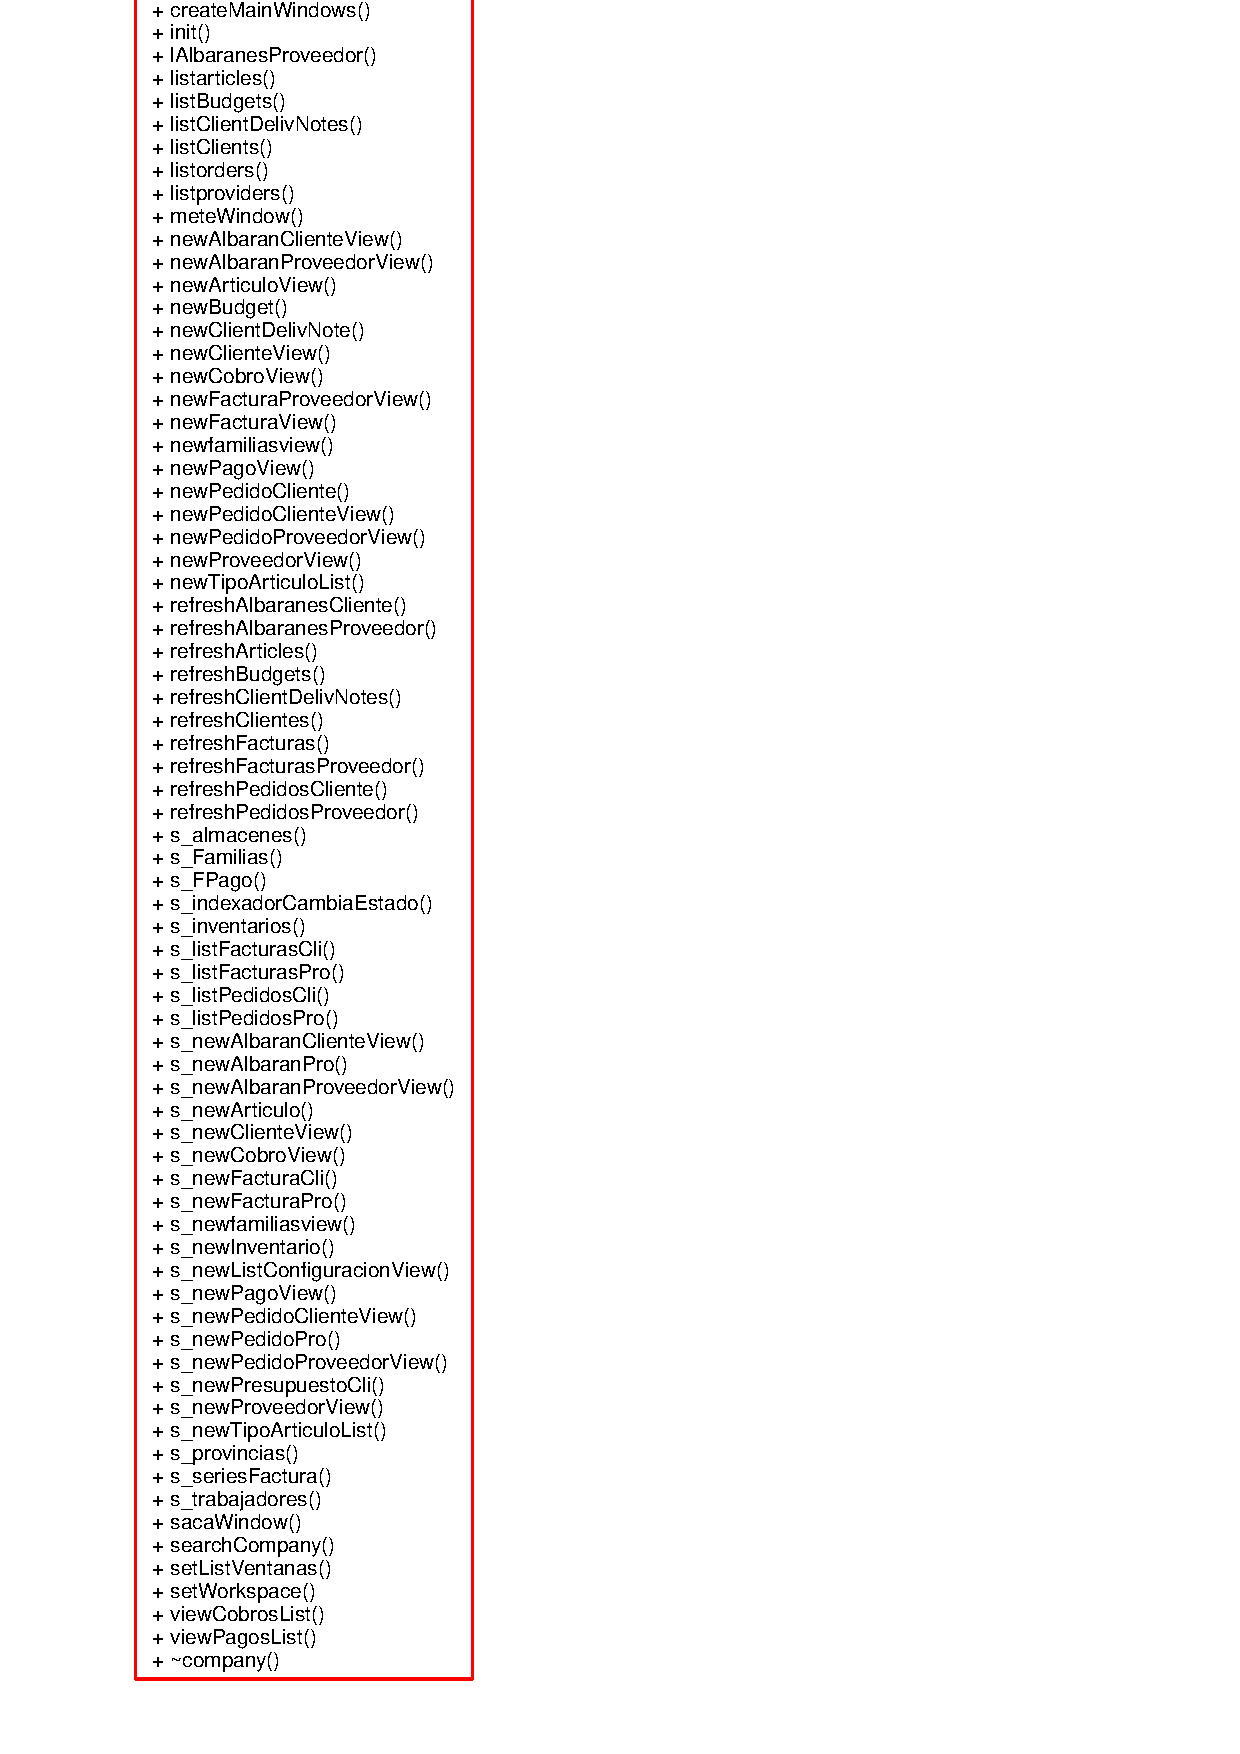
\includegraphics[width=131pt]{classArticuloList__coll__graph}
\end{center}
\end{figure}
\subsection*{Tipos p\'{u}blicos}
\begin{CompactItemize}
\item 
enum {\bf edmode} \{ {\bf Edit\-Mode} =  0, 
{\bf Select\-Mode} =  1
 \}
\end{CompactItemize}
\subsection*{Slots p\'{u}blicos}
\begin{CompactItemize}
\item 
virtual void {\bf on\_\-m\_\-filtro\_\-text\-Changed} (const QString \&text)\label{classArticuloList_i0}

\item 
virtual void {\bf on\_\-mui\_\-actualizar\_\-clicked} ()\label{classArticuloList_i1}

\item 
virtual void {\bf on\_\-mui\_\-borrar\_\-clicked} ()\label{classArticuloList_i2}

\item 
virtual void {\bf on\_\-mui\_\-configurar\_\-toggled} (bool checked)\label{classArticuloList_i3}

\item 
virtual void {\bf on\_\-mui\_\-crear\_\-clicked} ()\label{classArticuloList_i4}

\item 
virtual void {\bf on\_\-mui\_\-editar\_\-clicked} ()\label{classArticuloList_i5}

\item 
virtual void {\bf on\_\-mui\_\-exportar\_\-clicked} ()\label{classArticuloList_i6}

\item 
virtual void {\bf on\_\-mui\_\-importar\_\-clicked} ()\label{classArticuloList_i7}

\item 
virtual void {\bf on\_\-mui\_\-imprimir\_\-clicked} ()\label{classArticuloList_i8}

\item 
virtual void {\bf on\_\-mui\_\-list\_\-cell\-Double\-Clicked} (int, int)\label{classArticuloList_i9}

\item 
virtual void {\bf on\_\-mui\_\-list\_\-custom\-Context\-Menu\-Requested} (const QPoint \&)\label{classArticuloList_i10}

\item 
virtual void {\bf on\_\-mui\_\-list\_\-toogled\-Config} (bool check)\label{classArticuloList_i11}

\item 
virtual void {\bf s\_\-imprimir1} ()\label{classArticuloList_i12}

\end{CompactItemize}
\subsection*{Se\~{n}ales}
\begin{CompactItemize}
\item 
void {\bf selected} (QString)\label{classArticuloList_l0}

\end{CompactItemize}
\subsection*{M\'{e}todos p\'{u}blicos}
\begin{CompactItemize}
\item 
{\bf Articulo\-List} ({\bf company} $\ast$, QWidget $\ast$parent=0, Qt::WFlags flag=0, edmode editmodo=Edit\-Mode)\label{classArticuloList_a0}

\item 
void {\bf cargaconfig} ()\label{classArticuloList_a1}

\item 
QString {\bf codigocompletoarticulo} ()\label{classArticuloList_a2}

\item 
QString {\bf detalle\-Articulos} ()\label{classArticuloList_a3}

\item 
void {\bf edit\-Article} (int)
\item 
QString {\bf forma\-Query} ()\label{classArticuloList_a5}

\item 
void {\bf guardaconfig} ()\label{classArticuloList_a6}

\begin{CompactList}\small\item\em Funciones que se encargan en guardar y cargar la configuracion del listado. \item\end{CompactList}\item 
void {\bf hide\-Busqueda} ()\label{classArticuloList_a7}

\item 
QString {\bf id\-Article} ()\label{classArticuloList_a8}

\item 
QString {\bf idarticulo} ()\label{classArticuloList_a9}

\item 
void {\bf Imprimir} ()
\item 
void {\bf modoedicion} ()\label{classArticuloList_a11}

\item 
void {\bf modoseleccion} ()\label{classArticuloList_a12}

\item 
QString {\bf nomarticulo} ()\label{classArticuloList_a13}

\item 
void {\bf presenta} ()\label{classArticuloList_a14}

\item 
void {\bf show\-Busqueda} ()\label{classArticuloList_a15}

\end{CompactItemize}


\subsection{Descripci\'{o}n detallada}
Clase que maneja la lista de art\'{\i}culos. 



\subsection{Documentaci\'{o}n de las funciones miembro}
\index{ArticuloList@{Articulo\-List}!editArticle@{editArticle}}
\index{editArticle@{editArticle}!ArticuloList@{Articulo\-List}}
\subsubsection{\setlength{\rightskip}{0pt plus 5cm}void Articulo\-List::edit\-Article (int {\em row})}\label{classArticuloList_a4}


Si la carga no va bien entonces terminamos. \index{ArticuloList@{Articulo\-List}!Imprimir@{Imprimir}}
\index{Imprimir@{Imprimir}!ArticuloList@{Articulo\-List}}
\subsubsection{\setlength{\rightskip}{0pt plus 5cm}void Articulo\-List::Imprimir ()}\label{classArticuloList_a10}


Copiamos el archivo.

Copiamos el logo.

Linea de totales del presupuesto. 

La documentaci\'{o}n para esta clase fu\'{e} generada a partir de los siguientes archivos:\begin{CompactItemize}
\item 
articulolist.h\item 
articulolist.cpp\end{CompactItemize}
